Esta seccción corresponde a los resultados obtenidos con el problema descrito en el tutorial de Qiskit, recogido en la \textit{sección \ref{sec:4-tutorial de qiskit}}.

\begin{figure}[htbp]{}{Grafo del tutorial}
  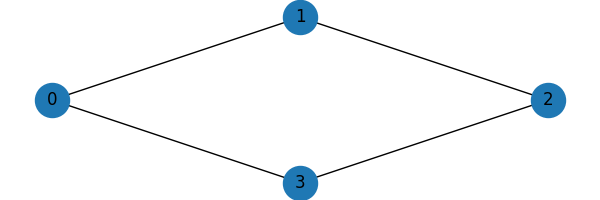
\includegraphics{qiskit-grafo/qiskit-grafo}
\end{figure}

Dada la naturaleza del problema Max-Cut existen siempre al menos dos resultados (en este caso ``1010'' y ``0101'') que devuelven el máximo de la función de coste (\(C(x) = 4\)).
Un resultado ``abcd'' sería equivalente a dar un valor ``a'' al nodo 3, ``b'' al nodo 2 y así sucesivamente.

\subsection{Resultados con QAOA}

\subsubsection{Estadísticas}

Las estadísticas obtenidas son las siguientes:

\begin{table}[htbp]{tab:5-tutorial-qaoa-estadisticas}{Resultados de la ejecución del problema \cite{qiskit_tutorial_antiguo}}
  \begin{tabular}{|c|r|r|}
    \hline
    \textbf{nº Capas} & \textbf{Estadística máxima (\%)} & \textbf{Estadística global (\%)} \\ \hline
    p = 1             & 100\%                            & 52.14\%                          \\ \hline
    p = 2             & 100\%                            & 98.17\%                          \\ \hline
    p = 3             & 100\%                            & 96.10\%                          \\ \hline
    p = 4             & 100\%                            & 98.70\%                          \\ \hline
    p = 5             & 100\%                            & 98.90\%                          \\ \hline
  \end{tabular}
\end{table}

Según esta tabla, se encuentra el camino óptimo con cualquier número de capas el 100\% de las ejecuciones.

Analizando los resultados, se concluye que son inmejorables, ya que siempre se encuentra el resultado óptimo y aumentar el número de capas disminuye la aparición de otros valores en la ejecución del algoritmo.

\subsubsection{Función gamma}

Se ha graficado la función gamma para poder visualizar posibles mínimos locales que se pudieran encontrar al ejecutar el optimizador clásico:

\begin{figure}[htbp]{}{Función gamma con \(\beta = 1.0\) y variando \(\gamma\)}
  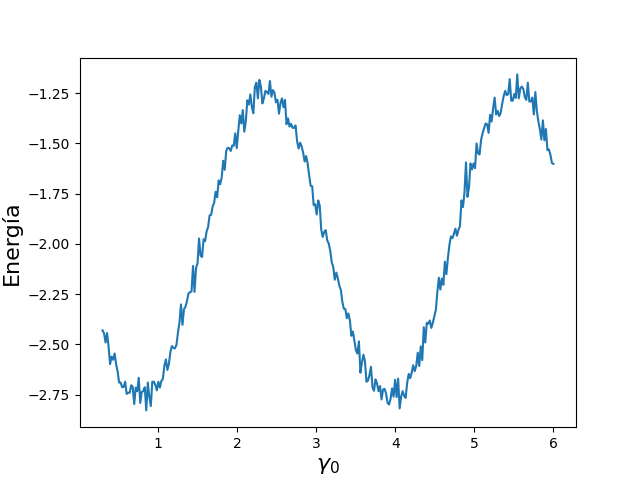
\includegraphics[scale=0.5]{qiskit-grafo/gamma-fun-2d}
\end{figure}

Como se puede ver, la función toma una forma sinusoidal y, como se ve en gráficas posteriores, tiene mucho menos ruido. Esto hace ver que el resultado óptimo es fácil de encontrar, lo que se ve reafirmado comprobando los resultados de la \textit{tabla \ref{tab:5-tutorial-qaoa-estadisticas}}.


%%% Local Variables:
%%% mode: latex
%%% TeX-master: "../tfgtfmthesisuam"
%%% End:
